\newcommand{\mydriver}{pdftex}

\documentclass[12pt,\mydriver]{thesis}

\usepackage{titlesec}
   \titleformat{\chapter}
      {\normalfont\large}{Chapter \thechapter:}{1em}{}

\usepackage{graphicx}
\usepackage{cite}
\usepackage{lscape}
\usepackage{indentfirst}
\usepackage{latexsym}
\usepackage{multirow}
\usepackage{tabls}
\usepackage{wrapfig}
\usepackage{slashbox}
\usepackage{longtable}
\usepackage{booktabs}
\usepackage{supertabular}
\usepackage{subeqn}
\usepackage{tikz}
\usetikzlibrary{arrows.meta}
\usepackage{listings}
\usepackage{slashbox}
\usepackage{subcaption}
\usepackage{verbatim}
\usepackage{graphicx}


%\usepackage[toc, page]{appendix}

\usepackage{color}
\usepackage{courier}
 
\definecolor{codegreen}{rgb}{0,0.6,0}
\definecolor{codegray}{rgb}{0.5,0.5,0.5}
\definecolor{codepurple}{rgb}{0.58,0,0.82}
\definecolor{backcolour}{rgb}{0.95,0.95,0.92}
 
\lstdefinestyle{mystyle}{
    backgroundcolor=\color{backcolour},   
    commentstyle=\color{codegreen},
    keywordstyle=\color{magenta},
    numberstyle=\tiny\color{codegray},
    stringstyle=\color{codepurple},
    basicstyle=\footnotesize,
    breakatwhitespace=false,         
    breaklines=true,                 
    captionpos=b,                    
    keepspaces=true,        
    language=Python,
    numbers=left,                    
    numbersep=5pt,                  
    showspaces=false,                
    showstringspaces=false,
    showtabs=false,                  
    tabsize=4
}
 
\lstset{style=mystyle}

\usepackage[bookmarks, colorlinks=true, plainpages=false, citecolor=blue, urlcolor=blue, filecolor=blue, linkcolor=blue]{hyperref}

\newcommand{\tbsp}{\rule{0pt}{18pt}} %used to get a vertical distance after \hlinewhat channel is
\renewcommand{\baselinestretch}{2}
\setlength{\textwidth}{5.9in}
\setlength{\textheight}{9in}
\setlength{\topmargin}{-.50in}
%\setlength{\topmargin}{0in}    %use this setting if the printer makes the the top margin 1/2 inch instead of 1 inch
\setlength{\oddsidemargin}{.6in}
\setlength{\parindent}{.4in}
\marginparwidth=0.6in
\pagestyle{empty}

\newcommand\eg[1]{e.g. {#1}}
\newcommand\ie[1]{i.e. {#1}}

\newenvironment{labeltable}{}{}

\begin{document}

%Abstract Page 

\hbox{\ }

\renewcommand{\baselinestretch}{1}
\small \normalsize

\begin{center}
\large{{ABSTRACT}} 

\vspace{3em} 

\end{center}
\hspace{-.15in}
\begin{tabular}{ll}
Title of thesis:    & {\large Identifying Extraneous Elements of Novice Source Code}
\ \\
&                          {\large Michael Patrick Neary III, Master of Science, 2018} \\
\ \\
Thesis directed by: & {\large  Professor Marie desJardins} \\
&  				{\large	 Department of Computer Science and Electrical Engineering} \\
\end{tabular}

\vspace{3em}

\renewcommand{\baselinestretch}{2}
\large \normalsize

Intelligent Tutoring Systems (ITS) are intelligent software systems that provide one-on-one guidance in a specific subject area. Introductory programming courses can use an ITS to give extra help to students learning to code for the first time. These systems generate constructive feedback to help the student understand the mistakes they make. Feedback is generated by analyzing correct programming solutions, looking for similarities with the student's code, to give a hint based on those similarities or lack thereof. The student's program might also have important information within its individual lines of code, as some such lines may be extraneous in the context of the problem. Current systems are not capable of meaningfully identifying these lines, or reasoning about it to give constructive feedback. I introduce a method for identification of extraneous lines of code, and show correct identification of extraneous lines in novice code artifacts.

 %(must be first, required, non-numbered)
%Titlepage

\thispagestyle{empty}
\hbox{\ }
\vspace{1in}
\renewcommand{\baselinestretch}{1}
\small\normalsize
\begin{center}

\large{Identifying Extraneous Elements of Novice Source Code}\\
\ \\
\ \\
\large{by} \\
\ \\
\large{Michael Patrick Neary III}%Your full name as it appears in University records.
\ \\
\ \\
\ \\
\ \\
\normalsize
Thesis submitted to the Faculty of the Graduate School of the \\
University of Maryland, Baltimore County in partial fulfillment \\
of the requirements for the degree of \\
Masters in Computer Science \\
2018
\end{center}

\vspace{7.5em}

\noindent Advisory Committee: \\
Professor Marie desJardins, Chair/Advisor \\
Professor Timothy Finin \\
Assistant Professor Cynthia Matuszek

 %(must follow Abstract, required, non-numbered)
%!TEX root = mainthesis.tex

\thispagestyle{empty}
\hbox{\ }

\vfill
\renewcommand{\baselinestretch}{1}
\small\normalsize

\vspace{-.65in}

\begin{center}
\large{\copyright \hbox{ }Copyright by\\
Michael Patrick Neary III  %Type your name as it appears in University records
\\
2018}
\end{center}

\vfill
 %(highly recommended, non-numbered)

%Pages from this point start at lower-case Roman number ii)
\pagestyle{plain}
\pagenumbering{roman}
\setcounter{page}{2}

% \include{Preface}  %(if present, start at lower-case Roman number ii)
% \include{Foreword} %(if present, lower-case Roman)
% %Dedication

\renewcommand{\baselinestretch}{2}
\small\normalsize
\hbox{\ }
 
\vspace{-.65in}

\begin{center}
\large{Dedication}
\end{center} 

If needed.
 %(if present, lower-case Roman)
% %Acknowledgments

\renewcommand{\baselinestretch}{2}
\small\normalsize
\hbox{\ }
 
\vspace{-.65in}

\begin{center}
\large{Acknowledgments} 
\end{center} 

\vspace{1ex}

Thanks for helping me, to be written. %(if present, lower-case Roman)

\renewcommand{\baselinestretch}{1}
\small\normalsize
\tableofcontents %(required, lower-case Roman)
%\newpage
%\listoftables %(if present, lower-case Roman)
%\newpage
%\listoffigures %(if present, lower-case Roman)
%\newpage
% LIST OF ABBREVIATIONS
% \addcontentsline{toc}{chapter}{List of Abbreviations}
% %List of Abbreviations

\renewcommand{\baselinestretch}{1}
\small\normalsize
\hbox{\ }

\vspace{-3em}

\begin{center}
\large{List of Abbreviations}
\end{center} 

AST - Abstract Syntax Tree
DDG - Directed Dependency Graph


\newpage
\setlength{\parskip}{0em}
\renewcommand{\baselinestretch}{2}
\small\normalsize

%Pages from this point start at Arabic numeral 1
\setcounter{page}{1}
\pagenumbering{arabic}
%!TEX root = mainthesis.tex
\renewcommand{\thechapter}{1}

\chapter{Introduction}
\section{Overview}

Intelligent Tutoring Systems (ITS) are a method of computer-based reinforcement of knowledge. They are capable of tracking student progress on a topic, and reinforcing that knowledge with constructive feedback. Recently, these systems have been used in introductory computer science classes. Intelligent Programming Tutors (IPT) are capable of helping students solidify their knowledge of computer programming by reinforcing concepts taught in a traditional lecture setting. The generation of meaningful hints in an IPT is difficult to do correctly. A successful IPT is capable of generating constructive feedback to guide the student towards the correct solution of a problem that they are working on.

Every problem has a particular goal in mind. Feedback to help reach that goal should be infrequent enough as not to coddle the student, but it should also be given exactly at the right time it is needed. Feedback should be informative enough to give insight into a misconception, but should not hand out the answer for free. Current methods to produce feedback include the comparison of the student's answer to past known solutions, or the generation of all possible solutions and searching through that space to find a similar solution. Each of these methods relies on a comparison to other programs, and do not inspect the student's program beyond that comparison. Therefore, they may fail to identify lines of code in a solution that are not necessary to accomplish the goal of a problem. I provide a method of identifying these extraneous lines of code so a hint generation system can use that knowledge to generate better feedback.

\section{Motivation}

If a student is given a problem to solve, they could use a variety of methods to produce a solution. Many different programs can produce the same solution to a problem. Therefore, generating hints based on the difference between a correct program and the student's current attempt can be limiting in the types of hints that are generated. This method of providing feedback guides students towards one particular method of solving the problem. However, the student's attempted solution could contain lines of code that are necessary for their solution to function, but are not necessary in what is considered correct. In fact, they could have lines of code that are unnecessary regardless of the correct solution used in current methods. I believe this to be an oversight in current hint generation systems: most methods simply ignore the potentially important information contained in unnecessary code.

\section{Research Problem}

I focus on the detection of extraneous lines of code in programs written by novice students. An \emph{extraneous} line of code is a line of code written in a program that does not have an effect on the desired solution to a problem. The majority of errors that students make when learning to program are syntactic \cite{Altadmri2015}, such errors are easily detectable by the compiler or interpreter of the language. An extraneous line of code is, by contrast, a \emph{semantic} error: \emph{the student may believe that writing that line of code has affected their desired solution, when in reality it has not.} Novice students are unable to accurately trace their programs linearly \cite{Kaczmarczyk2010}, which may contribute to the addition of meaningless lines of code. An unimportant line of code can contain valuable information about the misconception(s) that a student has on a particular topic, which is useful for generating meaningful hints. Identifying such lines of code is important to the acquisition of programming knowledge.

%It is important to note that although it would be useful to have information on extraneous lines when generating feedback that it does not make sense to give such feedback until after the student submits a complete solution. It  does not make sense to attempt to find lines of code that do not make sense if the solution itself is incomplete, as lines that might be considered extraneous may become important at a later point in time.


\section{Contribution}
In order to feasibly produce feedback from extraneous lines of code, I must be able to identify them programmatically and within a reasonable amount of time. I propose a system that is capable of identifying extraneous lines of code in a target program. The system utilizes artificial intelligence techniques and syntactical analysis to construct a graph of dependencies among lines of code. The single source, shortest path (SSSP) algorithm is applied to that graph to determine the lines that are not used between the start and end of a program.

% this chapter needs some kind of conclusion/wrapup and/or transition to the next chapter

%!TEX root = mainthesis.tex

\renewcommand{\thechapter}{2}

\chapter{Background}
The purpose of this chapter is to describe the components of Intelligent Tutoring Systems (ITS), and to give motivation for using ITS in programming courses. This chapter provides the necessary background knowledge on ITS, first-order logic, abstract syntax trees, and graph theory in order to understand the methodology in Chapter 4.

\section{Intelligent Tutoring}

An Intelligent Tutoring System (ITS) provides students with one-on-one guided instruction in a particular subject, typically after they have had prior exposure to that subject in a traditional classroom setting. A typical ITS mimics the interaction between a human tutor and a student. The goal of this interaction is to bring the student from a state of confusion in a subject to mastery of that subject. The ITS develops an internal model of what the student understands, providing the student with feedback based on that model to help guide the student towards mastery. The successful implementation of a tutoring system can be rewarding for both student and teacher, relieving some of the burden of teaching and learning in particularly difficult courses.

A majority of the content in introductory programming courses is difficult to grasp for the novice student, especially considering that the material is almost entirely novel. Those who fall behind in an introductory course are likely to suffer learned helplessness because each new concept builds upon previous concepts \cite{Jenkins2002}. Students also find it difficult to combine the basic structures of programming to form solutions to larger problems. If a student is able to think of a programmatic solution, they may still have trouble fixing bugs within that solution \cite{Lahtinen2005}. Students learn different concepts at different rates, which makes deciding what programming concepts to teach in what sequence particularly hard \cite{Rivers2016}. The programming instructor must find solutions for each these problems in order to be effective. The difficulty of programming for first-time learners and their instructors justifies the application of ITS to introductory programming.

An Intelligent Programming Tutor (IPT) is a specific implementation of an ITS for introductory programming. There are three important components of an IPT: domain knowledge, student knowledge, and tutoring knowledge. An IPT needs \emph{domain knowledge}, or a method of representing concepts related to programming (e.g., language syntax), in order to identify define content mastery. It needs a model of \emph{student knowledge}, or a method of encoding student understanding based on observation (e.g., code samples, multiple choice answers). An IPT also needs to know \emph{how to tutor}, or how to provide meaningful feedback to a student in a timely manner. Exceptional IPTs must have all three components, as constructive feedback is best generated from the combination of an accurate student model and sound domain knowledge. In this chapter, we discuss methods of modeling domain and student knowledge. The next chapter focuses on constructive feedback in-depth.

\subsection{Domain Knowledge}

It is imperative that an ITS has expert-level domain knowledge in the subject area it is applied to. An IPT needs knowledge of programming concepts in order to model what a student knows and to give feedback to that student. The necessary programming concepts for an IPT are how to write programs, how to identify and describe errors, and declarative information about programming structures \cite{Pillay2003}. These concepts should be encoded in an easily accessible manner, such that the student model and feedback generator can leverage the information. Programming domain knowledge need not be a separate entity in an IPT, although there are methods that rely on domain knowledge as a separate entity. One can easily incorporate domain knowledge into a student model or feedback generation method.

One direct method of domain knowledge representation utilizes first-order logic to create a knowledge base of programming concepts. This method views a solved programming problem as a conjunction of predicates that describe the expected constructs in an ideal solution. Weregama and Reye
\cite{Weragama2014} translated a set of student code examples into a knowledge base of correct solutions. They leverage this method of domain knowledge encoding to administer tutoring through simple planning algorithms. This method creates an accurate tutoring system, and is suited for handling the differences in solutions to problems.

Some IPTs encode domain knowledge as a graph to capture the relationship between programming concepts. Understanding the relationship among programming concepts is crucial for navigating the tutoring process in an IPT. If the system understands what the student has not yet mastered, and it knows the similar concepts that they do understand, it can generate feedback to bridge that gap. Kumar extends the graph of programming concepts, adding learning objectives to each concept \cite{Kumar2014}. Expert domain knowledge is the foundation of feedback generation and the internal student model.

\subsection{Student Knowledge}

It is important for the interaction between an intelligent tutor and a human to be as personalized as possible, since such a system must have an understanding of what the current user is capable of. It should reason from what it observes of the student's actions to determine the content that student has learned. This is a difficult task due to the inherent uncertainty in the observation of a student. A variety of methods for the representation of student knowledge that handle this uncertainty currently exist. A few of these methods utilize classic techniques such as Bayesian networks and Markov Decision Processes, while others employ novel methods. I first discuss the classic techniques applied to this problem, then more recent methods.

\todo{A variety of methods for the representation of student knowledge that handle this uncertainty currently exist}

\todo{give citations}
A Bayesian network is a directed acyclic graph used to encode conditional dependencies among random variables. These networks are the most utilized method for the modeling of student knowledge because they are easy to implement and they can determine the probability that some concept is understood given evidence, or lack thereof, for that hypothesis. Butz et al. use a Bayesian network to model the student who is using the system, and update their model based on the student's self-assessed understanding \cite{Butz2004}. Chang et al. go a step further by treating the student modeling problem as a function of time. This approach allows for the application of a dynamic Bayesian network. The model constructed is better than standard knowledge tracing, at the cost of an increase in training time \cite{Chang2006}.
%todo cite MDPs
A Markov Decision Process can also be used as a model for student behavior in a tutoring system. This technique determines an optimal policy for the intelligent tutor given a set of actions it can take (feedback to the student) and the states that result from taking those actions (student understanding of the material), with some probability that action A results in a transition from state S to S$'$. A student can be modeled using a Partially Observable Markov Decision Process (POMDP) because there is a level of uncertainty in the result of an action taken by a student. The model must do what it can with unreliable evidence, since a piece of feedback the student receives may either help or hurt their understanding of the topic. A student's response to a problem can vary, and it is not certain what state of understanding they are in until after their response is analyzed. A POMDP is a powerful modeling method, but the application of POMDPs can be intractable. Folsom-Kovarik et al. propose two variations---state queues and observation chains---of POMDPs to solve the problem of increased complexity in modeling student knowledge \cite{Folsom-Kovarik2013}. Both methods use properties of tutoring tasks to compress the information needed to reliably model a student with a POMDP. Their results show that their compression methods do not have any negative effect on the student model, but there was no substantial improvement over existing modeling methods.

% todo: *really* should clear up the last sentence or two: why is it there?
% todo: is the conclusion that this provides an efficiency boost but doesn't help (nor hurt) predictive performance?

%TODO: add a show section on hint generation?


\section{First-Order Logic}

My thesis uses the concept of first-order logic (FOL) to represent a particular kind of dependency among lines of code.  First-order logic statements utilize variables in order to describe objects and relationships in the world. These variables can be quantified: that is, one can write a statement that applies to every object or at least one object without naming anything specifically. A term in an FOL statement can be a constant, a variable, or a function. A constant is a symbol that represents a specific thing in the world. A variable can represent any object in the world. A function is a rule applied to one or more terms. Terms are used to write sentences, a predicate of n terms that evaluates to some truth, in FOL.

Complex sentences are created by joining terms with logical connectors, including conjunction ($\land$), disjunction ($\lor$), or implication ($\rightarrow$). Sentences can be quantified either universally ($\forall$, ``for all") or existentially ($\exists$, ``there exists"). The universal quantifier applied to a variable in a sentence is an assertion that the sentence is satisfiable by all members of the variable's domain. The existential quantifier on the same variable and sentence is an assertion that the sentence is satisfied by at least one member of its domain. As an example, consider the following English sentence: \emph{``All graduate students are tired.''} This is a blanket statement about all graduate students; therefore, a universally quantified sentence is necessary. The translation of this English sentence in FOL could look like this: $\forall x \ GradStudent(x) \Rightarrow \ Tired(x)$. In this sentence, the variable $x$ has the domain of people. This sentence is read as, ``For all people, if that person is a graduate student then they are tired.'' A group of sentences can be written to describe a system, and subsequently reasoned over to prove different sentences related to that system.

%\emph{``Anyone who has graduated and has a job is happy.''} This is a complex statement that applies to anyone, so an existential quantifier is necessary. Taking x to have the domain of all people again, in FOL this statement is: $\exists x \ Graduated(x) \land hasJob(x) \Rightarrow happy(x)$. This is read as ``There exists some person who if they have graduated and have a job then they are happy.''

FOL is used to prove statements about the world based on what is already known or observable. Observed facts and known rules can be combined into a collection of sentences known as a knowledge base (KB). The KB is a collection of statements about the world. A model of a KB is an assignment of True/False values to each symbol in the KB. Given a model, the conjunction of each evaluated sentence under that model results in an over all KB evaluation to True or False. KB evaluation is important to determining logical entailment.

The logical entailment of a sentence S by a KB, denoted by $KB \models S$, occurs when every model that evaluates KB to True also evaluates S to be True. That is to say that the sentence S is a logical consequence of the knowledge base. Resolution is used to check if $KB \models S$. This process attempts to prove that no model exists such that $KB \land \lnot S$ evaluates to True. Resolution is performed by applying logical inference rules to the previous conjunction. If a contradiction arises during the application of logical inference then that proves $KB \models S$.

%TODO: MUST EXPLAIN **WHY** FOL IS NECESSARY!!!!!

\section{Graphs}
A graph, sometimes referred to as a network, is a mathematical construct used to describe a relationship among objects. A graph G is comprised of two sets (V, E), which correspond to vertices and edges. Each vertice, or node, represents one particular object. Each edge is a pair of vertices (u, v) that represents a connection between two objects. The edges of a directed graph go one way from the source node (u) to the destination node (v), whereas an undirected graph's edges are bidirectional. A relevant problem to this thesis is that of shortest paths.

A number of relationships exist within a computer program, where single instructions interact with data or with other instructions to accomplish a particular goal. A program can be represented as a graph where nodes correspond to line numbers of individual instructions and edges correspond to an interaction that takes place between two instructions.

\subsection{Single Source Shortest Path}
Given a directed graph G = (V, E), a path from a starting node to a destination node is a sequence of nodes in V such that each pair of adjacent nodes in the sequence are connected by an edge in E. The problem of shortest paths (SSSP) is finding the path of minimal length from a starting node to a goal node. The problem of single source shortest paths is finding every shortest path from some beginning node to every other node in the graph.

%TODO: MUST EXPLAIN **WHY** SSSP IS RELEVATNT TO MY THESIS
%TODO: algorithm description and/or graph example figure here

\section{Abstract Syntax Trees}
Formal representation of language syntax and structure is useful at compile time and for general analysis of program structure. An abstract syntax tree (AST) encodes the syntactical structure of source code as a tree; i.e., an undirected graph where any pair of vertices have exactly one path that connects them. Each node of an AST represents an abstract programming construct within the source, such as statements, expressions, or decisions. An AST disregards portions of the actual syntax since some constructs, like grouping of parentheses, can be derived from the tree structure itself.

%TODO: MUST EXPLAIN **WHY** ASTs ARE RELEVANT TO MY THESIS
%TODO: AST example figure here

%!TEX root = mainthesis.tex

\renewcommand{\thechapter}{3}
\chapter{Related Work}
In this chapter, I provide related work in the generation of constructive feedback for Intelligent Programming Tutors. I discuss the strengths and drawbacks of each method.

\section{Constructive Feedback}

Quality feedback is important to facilitate the acquisition of new knowledge. The majority of feedback that a new programmer receives comes from the compiler or interpreter of the language they are using, which can be hard to decipher. This type of feedback is useless to the novice beyond highlighting syntax errors. It is therefore up to the instructor to provide meaningful feedback on student programming work, ranging from proper syntax use to walking through flawed logic. An IPT removes the need for the instructor to intervene and correct a flaw in student thinking. It should provide meaningful hints towards valid solutions and correct explanations of errors that arise when programming.

Stamper et al. laid the groundwork for constructive feedback in an intelligent tutor with the Hint Factory \cite{Stamper2013}. They created a system for a logic tutor that could generate step-by-step hints as a student was attempting to solve a problem. This system used data from past student problem solving attempts to create a Markov Decision Process, effectively creating a student model that was not individualized. Using this model, the system would figure out what the next best problem solving state was, and generate a hint to get the student into that state. Through the use of this hint generation method, Stamper et al. found that students increased the number of times they attempted to answer questions, and increased the number of questions they solved overall. The students who used the hint generation system achieved higher scores on post-tests in their experiments and received higher course grades overall. The Hint Factory was meant to be generalizable to all sorts of intelligent tutors, but there are limitations to using this system in a tutoring environment for programming.
%TODO: GO BACK TO THE HINT FACTORY PAPER AND NAME THE LIMITATIONS THAT IT PROPOSES

Generating hints for a student trying to solve a programming problem can be difficult. The solution space for a single programming problem can be infinitely large unless a bound is placed on the syntax or standard library functions that are allowed in a solution. Searching through a solution space to find the most similar solution to what a student has is therefore impractical. Current methods for hint generation in this space either circumvent the need for looking at the solution space, or take steps to pare down its size.

There have been a few approaches for improving hint generation and programming feedback in an IPT. Recently, there has been a push towards the use of programming data to generate feedback. One method was developed by Lazar and Bratko without the need for a state-space representation of the problem solving process, instead analyzing student programs by looking for common “edits” between them \cite{Lazar}. Once these edits were found, the authors applied them to a student submission until a proper solution was reached. From the sequence of applied edits, they derived hints they would show to the student. Using this approach, they were able to fix 70\% of student submissions, independent of language choice, without the need to manually enter common mistakes for the system to be aware of.

Other approaches treat the problem solving environment of learning to program with a state-space representation method. Koedinger et al. generate a solution space using Abstract Syntax Trees created from correct student code samples, and they reduce the size of this solution space by applying certain transformations on these ASTs \cite{Koedinger2013}. Using the reduced solution space, they create the AST for a student's intermediate submission, and then compute the difference between the intermediate solution and the known solutions. The goal is then to reverse the differences to generate feedback from the closest solution found.

Expanding on their previous results, Rivers and Koedinger describe a path construction method, where instead of comparing all possible solutions, they develop a space of possible paths that a student may take in order to get to a solution, and generate hints based on the most likely path that a student could take, given the previous attempts \cite{Rivers2016}. This method was more computationally feasible than generating the solution space, and they found most hints to be generated fairly quickly (in less than one minute). However, they are not certain how helpful the hints generated were for the students interacting with the system.

%!TEX root = mainthesis.tex
\renewcommand{\thechapter}{4}
\chapter{Methodology}
My process for detecting extraneous lines of code is composed of two parts: the detection of line dependencies and the determination of program correctness. This chapter discusses the methods I use to uncover dependencies among lines of code in a given program. I also discuss the process of determining the correctness of a solution. Combining both line dependencies and program correctness, I describe a method for identifying extraneous lines of code.

\section{Line Dependencies}
%Static and dynamic code analysis tools can analyze the flow of data and control throughout the life cycle of a program. These tools can determine metrics such as code coverage for software developers.
The execution of a single line of code in a program depends on the outcome of at least one line of code that came before it. This is a quality shared by all programs, and it can be leveraged to find extraneous lines of code. The following section outlines three different types of line dependencies necessary to find such extraneous code.

Understanding how data flows through a program helps to determine what computations are necessary to fulfill the program goal.

\subsection{Data Dependencies}
The first type of line dependency is the data dependency. This line dependency is defined as a relationship between two lines of code where each line uses the same piece of information in a specific manner. As a program executes, it stores data in variables and uses those variables for various computations. This dependency occurs between a line that assigns or alters the value of a variable, and a line that uses the contents of that variable in some manner. The line that edits a value must come before a line that uses that value. Two lines that use the same value in different computations do not constitute a data dependency, since data isn't flowing between those two lines: it is only being looked up. When a variable is updated, any line that uses that value later would be depended upon the line that performed update and not on any previous lines that altered that same variable. 

Formally, a data dependency exists between two lines $(a,b)$ if and only if the following is true: line $a$ comes before line $b$ in the source code; there is an identifier $x$ that exists on both line $a$ and line $b$; line $a$ is an assignment of a value to identifier $x$; and line $b$ uses identifier $x$ is a way that is not an assignment. This definition is easily written in FOL in Equation 4.1:
\begin{equation}
\exists a,b,id \ Depends(a,b) \leftrightarrow isBefore(a,b) \land Assigns(a, id) \land Uses(b, id)
\end{equation}
The domains of $a,b$ are all possible line numbers (as integers) in the target program. The domain of $id$ is all possible variables that are initialized at any point in the target program. Each relationship between $a,b$ represents a fact about the interaction between those two lines. $isBefore(a, b)$ encodes the fact that line $a$ comes before line $b$ in a piece of source code. $Assigns(a, id)$ encodes the fact that line $a$ contains the assignment of a value to identifier $id$. $Uses(b, id)$ encodes the fact that line $b$ needs id $id$ in order to execute.

\subsection{Structural Dependencies}
%The second type of line dependency is the structural dependency. This type of dependency occurs within lines of code that are a part of the same programmatic structure. These structures include constructs like the if statement, for loop, while loop, or function definition. A structural dependency describes the relationship among the lines of code between themselves in a given structure and in relation to the rest of the program. For example, all the lines within the body of an If-Else statement are dependent upon the line that hold the condition for that If statement, as well as all the lines within the body of the Else clause.

The second type of line dependency is the structural dependency. This type of line dependency is defined as the relationship between a line of code and the programming construct that encloses it. There are a few programming structures that enclose blocks of code, such as the if statement, for loop, or while loop. The only way that a line of code enclosed by one of these programming structures will execute is when the entry point of that structure is triggered. For example, the lines of code enclosed by an if statement will only execute if the condition of that statement is True. Therefore, a structural dependency exists between the line of that condition and each line of the if statement's body, as the body would not execute without first testing the condition. A similar argument can be made for the iterative structures For and While.



%TODO: the above section is "not very clear" according to Marie

\subsection{Execution Dependencies}
This is the most straightforward type of line dependency. A program is simply a sequence of lines of code that execute one after another. It can be said that a dependency exists between each the each pair of lines in the chain of execution. That is to say that if line A is executed in a program's life cycle, followed by line B, then a dependency exists between line A and line B. This type of line dependency is used to determine the usefulness of other types of line dependencies. It is important to note that using only execution dependencies to detect extraneous lines is not enough.

%TODO: **WHY** is it not enough?? Last few sentences confusing.

\subsection{Code Coverage and Dead Code}
An analysis of only the executed lines of a program does not provide enough information for the detection of extraneous lines of code. Discovery of \emph{dead code} --- i.e., lines of code that are never executed --- depends on the analysis of program execution. Tools for the discovery of dead code are an important part of the software development life cycle, but are not sufficient for extraneous line detection. In the IPT domain, novice programmers often write lines of code that are executed by the machine but do not contribute to the overall goal of the program. As seen in Figure \ref{fig:deadcodecounterexample}, if a student initializes a variable in a global scope that they fail to use in the remainder of their program, that code would not be caught by analyzing the executed lines of that program. The line that contains that variable's assignment will be executed every time, and thus not be deemed extraneous even though it does not affect the overall goal of that program.
\begin{figure}
\begin{lstlisting}
CONST_VAR = 45

def main():
    x = int(input(`Enter an integer:'))
    print(`:) ' * x)

main()
\end{lstlisting}
\caption{Line 1 is executed, but it is not used anywhere else in the program. If execution dependencies are used, Line 1 would be incorrectly identified as not extraneous.}
\label{fig:deadcodecounterexample}
\end{figure}

% Might not need an execution line dependency example, I think this is pretty straightforward.
%TODO: Consider describing execution line dependencies first.


\section{Uncovering Line Dependencies}
In order to identify extraneous lines of code, we must first detect each of the three types of line dependencies. Data dependencies are the most computationally difficult to detect, followed by structural and execution dependencies. The process of detecting each of the described dependencies is discussed in the following sections.

\subsection{Detecting Data Dependencies}

The detection of data dependencies logically follows from the formal definition. First order logic resolution is applied to a knowledge base in order to determine the lines of code that are dependent upon each other. The target program must first be converted into a knowledge base. To begin this process, the $isBefore$ relationship is added to the knowledge base for every line number with every other line number that occurs afterwards. The target program is then transformed into an AST. This encoding standardizes the target program to make certain relationships easier to find than processing the original source.

%TODO: Math mode and FOL functions do not play nice... find a better way?

The AST is traversed node-by-node to find the lines that contain data assignment and usage. Each time that an identifier is assigned a value at a node on the AST, the $Assigns$ relationship between the line number of that node and the referenced identifier is added to the knowledge base. This relationship signifies that the identifier is assigned a value on that line, but the actual value of the assignment is not relevant to the dependency. It only matters that the identifier becomes a part of the program at that line. Each time that an identifier appears on a line other than when is it assigned a value, such as in an expression or in an argument to a function call, the $Uses$ relationship is added to the knowledge base. This relationship between the line number and the identifier signifies that the identifier is used in some manner on that line. The actual usage of that identifier is not relevant to the dependency; only the fact that is was used in some manner is relevant. After traversing the AST, the knowledge base contains every instance where an identifier is assigned a value or used in some manner in the form of a fact.

The knowledge base is now usable as it contains all the necessary facts to determine the data dependencies. First-order logic resolution is applied to determine all possible pairs of line numbers $(a,b)$ that satisfy Equation 4.1. This process results in a list of every data dependency that exists in the target program.

\subsection{Detecting Structural Dependencies}
A structural dependency exists among two lines $(a,b)$ if they are both used in the same programming structure, independent of the contents of each line. The structural dependencies of the programming structures available to the novice student look similar. It is possible to define this type of dependency for all programming structures, but I limit the definition to three basic structures known to all students within the first few weeks of an introductory course. The dependencies within Conditionals, For Loops, and While Loops are defined in the next sections.

The structural dependencies in conditional statements are straightforward. The body of an If statement will only execute if the condition of that statement is true. Regardless of how that condition evaluates at run time, every line in the body of an If statement is structurally dependent on the line that contains the condition. Similarly, if there is an attached Else clause, every line in the body of that clause is dependent on the condition. The Else If clause is similar, except every line in the body of that clause is only dependent upon the condition of the Else If and not any preceding conditions.

%todo{figures for each of the structural dependencies are needed}

\subsection{Detecting Execution Dependencies}
The detection of execution dependencies can be performed with existing code tracing solutions, usually used for debugging software. A code tracer executes source code one line at a time, reporting the time and order in which lines are executed. This report is used to say that an execution dependency exists when a line $b$ is executed immediately after another line $a$.

\subsection{Directed Dependency Graph}
A method to successfully detect each type of line dependency has been described, but that detection alone is not sufficient for finding extraneous lines. The next step to find extraneous lines is the selection of an appropriate data structure. A line dependency is a one-way relationship between two line numbers, resembling an edge in a directed graph. Intuition suggests that a directed graph of line dependencies would allow the discovery of a path through dependencies as a program executes. The idea of tracing through dependencies to find extraneous lines motivates the construction of a directed dependency graph (DDG) from every known line dependency in the target program.

To build the DDG, start from the target program itself. For each valid line number in the target program, add a node to the graph. Add an edge for each detected dependency $(a,b)$ among lines. The source of this edge must be $b$, and the destination of this edge must be $a$. It is now possible to perform searches and path-finding over the underlying dependencies in the target program.

Here is a simple program, and the resulting DDG without execution dependencies:
\begin{figure}
\centering
\begin{minipage}{.5\textwidth}
\centering
\begin{lstlisting}
var1 = 3
var2 = 15
val = var1 + var2
if val % 2 == 0:
    print(`even')
else:
    print(`odd')
\end{lstlisting}
\end{minipage}%
\begin{minipage}{.5\textwidth}
\begin{tikzpicture}
\begin{scope}[every node/.style={circle,thick,draw}]
\node [draw, circle] (1) {1};
\node [draw, circle] (2) [right of=1] {2};
\node [draw, circle] (3) [right of=2] {3};
\node [draw, circle] (4) [right of=3] {4};
\node [draw, circle, red] (5) [right of=4] {5};
\node [draw, circle] (6) [right of=5] {6};
\node [draw, circle, red] (7) [right of=6] {7};
\end{scope}

\begin{scope}[>={Stealth[black]}]

\draw [->, thick] (3.north) to [out=135, in=45] (1.north);
\draw [->, thick] (3.south) to [out=-135, in=-45] (2.south);
\draw [->, thick] (4.south) to [out=-135, in=-45] (3.south);
\draw [->, thick] (5.south) to [out=-135, in=-45] (4.south);
\draw [->, thick] (6.north) to [out=135, in=45] (4.north);
\draw [->, thick] (7.south) to [out=-135, in=-45] (6.south);

\end{scope}
\end{tikzpicture}
\end{minipage}
\caption{A short program, and the derived DDG without execution dependencies.}
\end{figure}

Here is that same program, and the resulting DDG with execution dependencies:
\begin{figure}
\centering
\begin{minipage}{.5\textwidth}
\centering
\begin{lstlisting}
var1 = 3
var2 = 15
val = var1 + var2
if val % 2 == 0:
    print(`even')
else:
    print(`odd')
\end{lstlisting}
\end{minipage}%
\begin{minipage}{.5\textwidth}
\begin{tikzpicture}
\begin{scope}[every node/.style={circle,thick,draw}]
\node [draw, circle] (1) {1};
\node [draw, circle] (2) [right of=1] {2};
\node [draw, circle] (3) [right of=2] {3};
\node [draw, circle] (4) [right of=3] {4};
\node [draw, circle, red] (5) [right of=4] {5};
\node [draw, circle] (6) [right of=5] {6};
\node [draw, circle, red] (7) [right of=6] {7};
\end{scope}

\begin{scope}[>={Stealth[black]}]

\draw [->, thick, blue] (3.north) to [out=135, in=45] (1.north);
\draw [->, thick, blue] (3.south) to [out=-135, in=-45] (2.south);
\draw [->, thick, blue] (4.south) to [out=-135, in=-45] (3.south);
\draw [->, thick, green] (5.south) to [out=-135, in=-45] (4.south);
\draw [->, thick, green] (6.north) to [out=135, in=45] (4.north);
\draw [->, thick, ] (7.south) to [out=-135, in=-45] (6.south);
\draw [->, thick] (5) to (4);
\draw [->, thick] (4) to (3);
\draw [->, thick] (3) to (2);
\draw [->, thick] (2) to (1);

\end{scope}
\end{tikzpicture}
\end{minipage}
\caption{A short program, and the derived DDG with execution dependencies.}
\end{figure}

\section{Program correctness}
The next step in detecting extraneous lines of code is determining the line in the target program that is responsible for outputting the correct solution. For this step, I assume that the target program is in a final state. A final state proposes a solution to the problem it was written for, producing an output for every input given to it. I assume a final state due to the uncertain nature of extraneous lines of code. A program may contain lines of code that do not contribute to the output before it is complete. These lines may end up tying into the solution after more code is written. Also, computing the dependencies can be costly for large programs as it involves both program tracing and recursion over an AST. Therefore, it is not reasonable to detect extraneous lines of code unless the target program is in a final state. With this assumption, a target program is correct if it is in a final state, and it satisfies every goal of the problem it is intended to solve

The goal of a particular target program is defined prior to performing the extraneous line detection process. A goal defines what that program is trying to accomplish in order to determine if a given solution is correct. Typically, the goal of a small program written by a novice is to output some value given some input. The exact mapping from input to output is usually given in an assignment description. For example, a student may be asked to take an integer as an input, and output whether or not that integer is even. Programs can have multiple goals if there are multiple tasks for a student to perform. In the previous example, the student could also have to write a value to the screen a certain number of times. Multiple goals need not be satisfied for the same input as different inputs might illicit different outputs. For example, the target program could be a currency converter that takes an amount in US Dollars and outputs that amount in Canadian Dollars. The goals for a program should be defined on an input-by-input basis in order to reflect the correct result given a particular input. Defining the program goals allow us to determine where in the target program that solution is finalized.

\subsection{Matching Code Lines to Output}
After defining the goals of the target program, it is necessary to determine which lines of the source code are responsible for producing its output. This step is done by running the student's code through a program tracer. The output of the tracer in a combination of the output of the program immediately preceded by the line of code that executed before the output was produced. For each line that produces an output as determined by the tracer, I add a relationship between the line number and the contents of the output as a fact to the KB. Each line number and string content pair as given the $hasOutput$ relationship.

\section{Reporting Extraneous Lines}
%TODO: This section needs to be redone as it is hard to follow.
A target program has been manipulated in such a manner that makes the detection of extraneous lines simple. If the line responsible for a particular output is known, this method is able to trace backwards through the dependencies of that line in the DDG. The dependency edges were added with $b$ as the source to help with this backwards tracing step. An extraneous line of code does not appear on a path from the solution line to any node above that line. That is, an extraneous line of code was not used to arrive at a particular output. To ensure accuracy, the path from the solution line to every line that occurs before it is checked. This is done by performing the single source shortest path algorithm for each identified output line.
%TODO: why/how does SSSP work in this context?

%\renewcommand{\thechapter}{5}
\chapter{Experimentation}
This chapter discusses the methods of experimentation that are used to analyze student solutions to programming problems, including the human labelers, their qualifications, and their overall agreement on the data sets.

\section{Data}
The data that I use to test my method of extraneous code detection originates from the Computer Science I for Majors (CMSC 201) course at the University of Maryland, Baltimore County (UMBC). This is the first course in programming, required for Computer Science majors at the university. The course is taught in Python, a suitable beginner's programming language. It is assumed that the students in this course do not have prior programming experience. Homework assignments during this semester were given weekly, with four to seven individual problems. I have collected several hundred code samples for two different problems that were given as homework assignments during the Fall semester of 2016. Each of these problems have been selected for their simplicity; they can be solved by applying a few fundamental programming structures. The following paragraphs are short descriptions of each of the problems used in this work.

\begin{figure}[ht]
\begin{lstlisting}[numbers=none]
def main():
    temp = float(input("Please enter the temperature: "))
    unit = input("Enter 'C' for Celsius, or 'K' for Kelvin: ")
    if unit == "K":
        temp -= 273.15
    
    if temp >= 100:
        print("At this temperature, water is a gas.")
    elif temp <= 0:
        print("At this temperature, water is a solid.")
    else:
        print("At this temperature, water is a liquid.")

main()
\end{lstlisting}
\caption{A correct solution for Problem 1.}
\label{fig:correctp1}
\end{figure}
\subsection{Problem 1: State of Matter}
The goal of this problem is to output the state of matter that water would be in at a certain temperature. This problem asks the student to accept two inputs from the user: a floating point number that represents a temperature, and a character to determine what unit that temperature is in (`C' for Celsius or `K' for Kelvin). Their program must output the state of matter that water would be in at the given temperature. Acceptable output should contain one of the following strings: `liquid', `solid', or `gas.' The output format was not strictly enforced, as long as it produced the correct string for the given input. An appropriate solution uses two input statements, followed by a sequence of condition statements, to produce correct output. Refer to Figure \ref{fig:correctp1} for a correct solution.


\begin{figure}[ht]
\begin{lstlisting}[numbers=none]
def main():
    width = int(input("Enter the width of the box: "))
    height = int(input("Enter the height of the box: "))
    outline = input("Enter a symbol for the box outline:")
    fill = input("Enter a symbol for the box fill:")

    for i in range(width):
        print(outline, end = "")
    print()
    
    if height > 1:
        for i in range(height - 2):
            print(outline, end = "")
            
            if width > 1:
                for j in range(width - 2):
                    print(fill, end = "")
                    
                print(outline, end = "")
            
            print()

    for i in range(width):
        print(outline, end = "")
    
    print()

main()
  \end{lstlisting}
  \caption{A correct solution for Problem 2.}
  \label{fig:correctp2}
\end{figure}

\subsection{Problem 2: Box Display}
The goal of this problem is to display a rectangular box on the screen constructed with any character on the keyboard. The problem asks the student to accept two integer inputs that represent the height and width of the box, one character input that fills the inside of the box, and one character input that makes up the border of the box. Their program must output a box with the given dimensions, constructed with the given characters in the correct places. A student must combine multiple programming structures to give a correct output as they must consider a few edge cases in order to produce a correct solution. Refer to Figure \ref{fig:correctp2} for a correct solution.

\subsection{Data Preprocessing}
Each of the data sets must be standardized before my extraneous line detection method is evaluated. Standardization of each file helps streamline the process of labeling the extraneous lines, both manually and automatically. The contents of each file in the same assignment group are different for each student, but the name of each submitted file is the same within each data set (i.e., hw3.txt). To distinguish between unique solutions within each data set, every file name is appended with a different number (hw3\_123.txt). Every file is stripped of the file header and comments to protect the identity of the student who submitted that file. Identity was not preserved between the datasets, meaning that hw3\_123.txt and hw5\_123.txt may not be the same student's code. All blank lines are removed from the file to remove the possibility of reporting such lines as extraneous. All empty files are removed from the dataset.

\section{Data Labeling}

Each individual assignment must be manually checked for extraneous lines of code in order to properly evaluate my detection method. This involves reading through each program, looking for lines of code that do not make sense or do not help the student solve the problem. I enlisted the help of four experienced undergraduate computer science students as domain experts to label these data independently of each other. Since I know the intricacies of my detection method, I would introduce bias into the data set if I were the only person assigning labels. I do not want to subconsciously label lines that I know would be detected and not label lines that I know would not be detected. Therefore, I did not have a role in the labeling process apart from getting these experts started. They were not given guidance on how to label any individual assignment; I only answered hypothetical questions before they began. The set up process involved an explanation of the definition of an extraneous line of code, an explanation of the two problems, and a brief explanation of the labeling web application.

\begin{figure}[ht]
  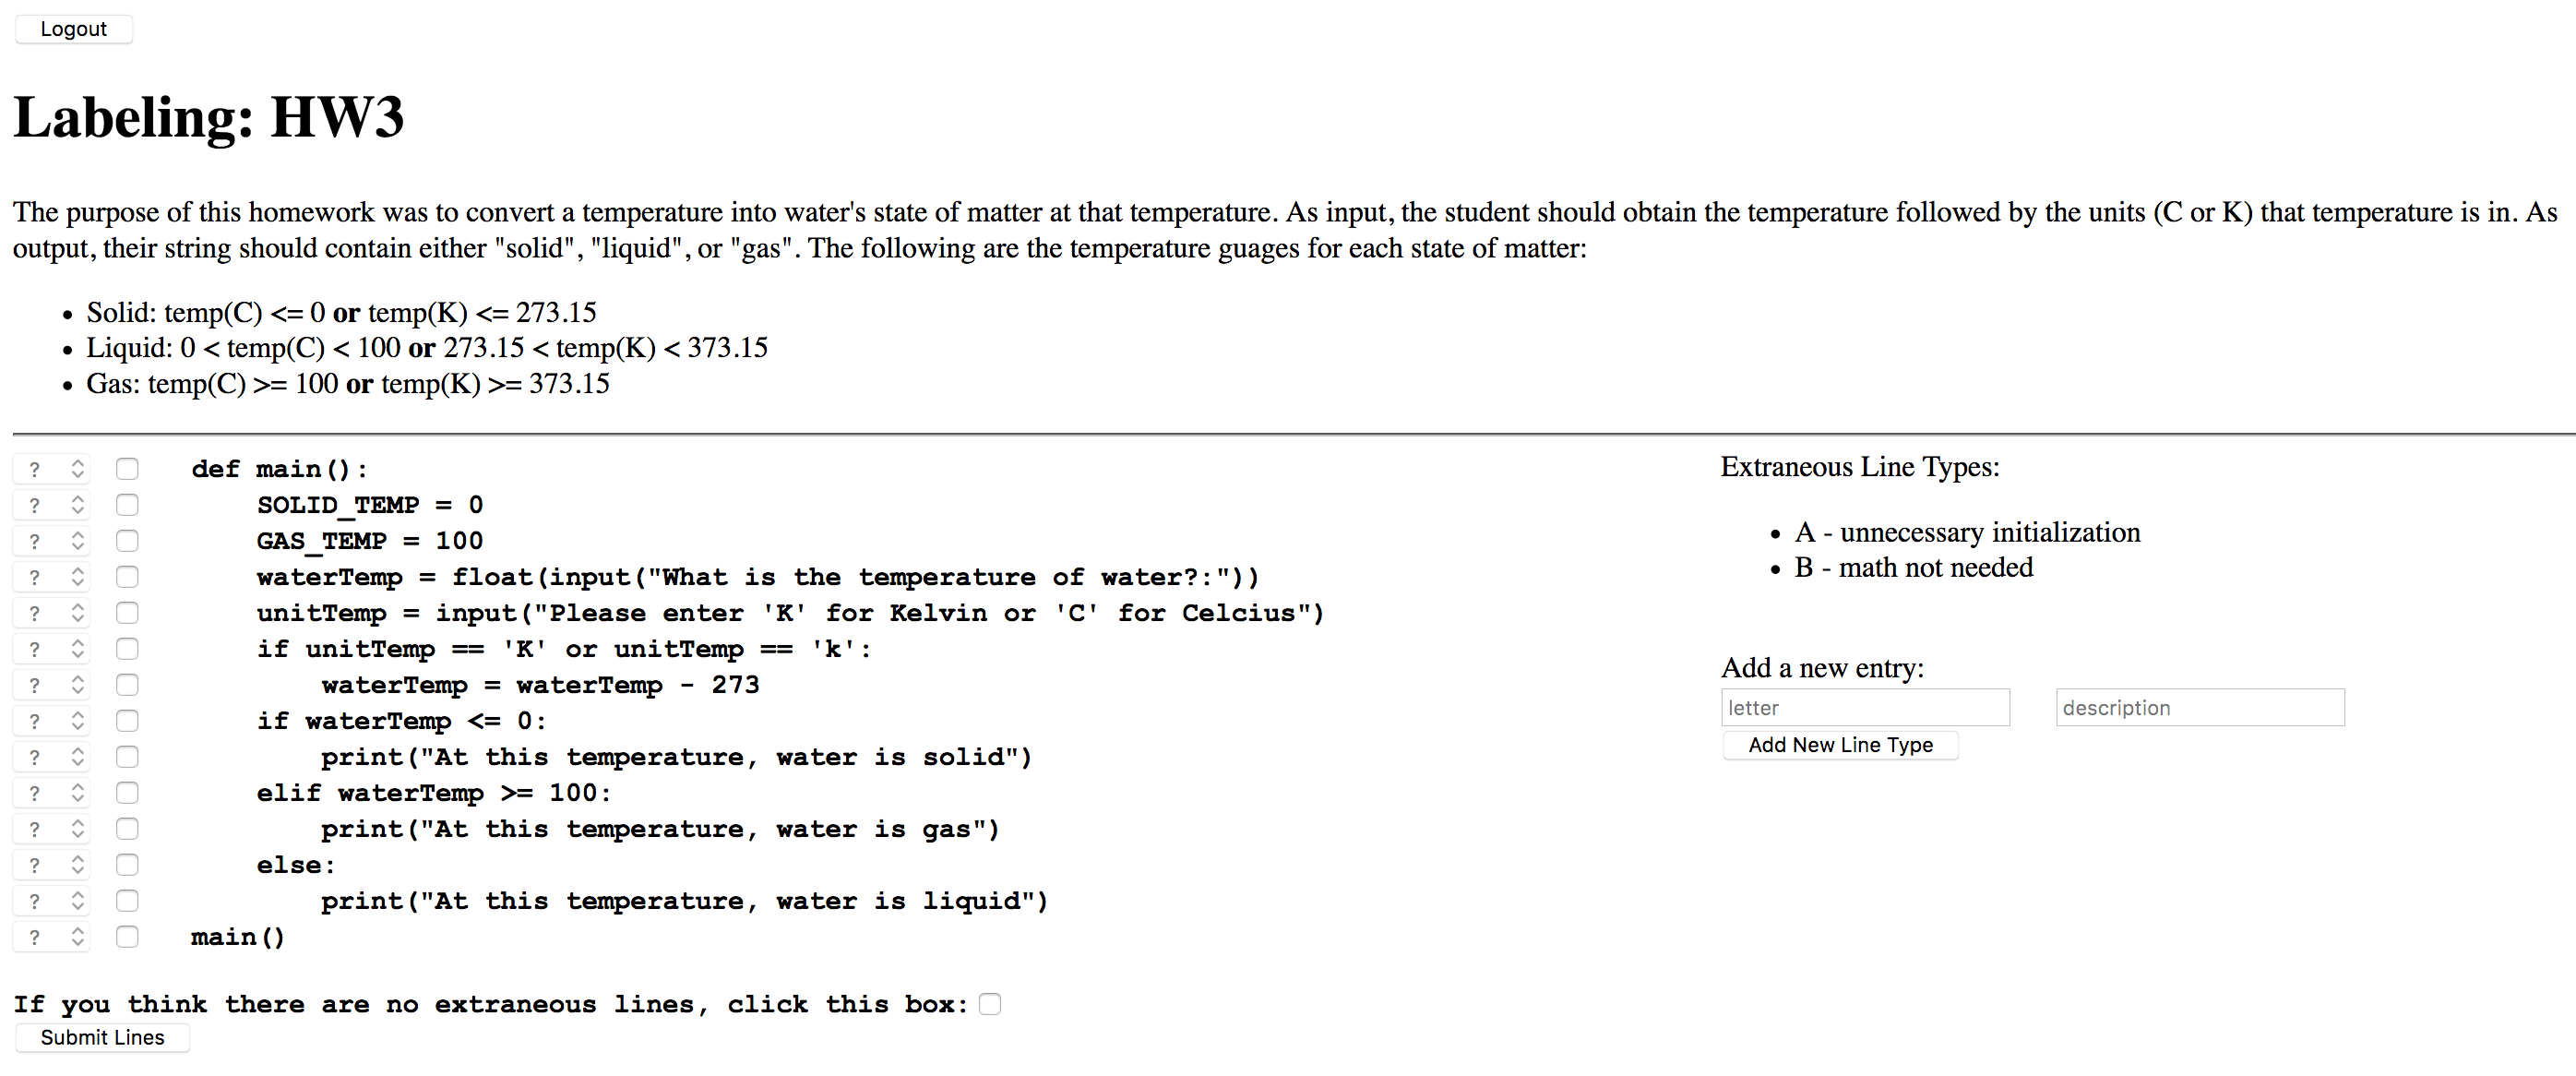
\includegraphics[width=\textwidth]{figures/webapp.png}
  \caption{Sample screen of a student labeling an assignment.}
  \label{fig:webapp}
\end{figure}

I built a custom web application to standardize the collection of labels. It allows me to easily collect different sets of labels from different people. Each user of the application reads each program, and determines which lines, if any, are extraneous. The application expedites the process of labeling, since navigating between assignments and keeping track of what has already been labeled is taken care of for the user. Figure \ref{fig:webapp} shows a sample screen for a single assignment. On the top of the page,there is a description of the problem, including any guidelines as to what constitutes a correct solution, for their reference. On the left-hand side of the screen, they can view the source code line-by-line. A line is marked as extraneous by clicking a checkbox next to the line in this area and choosing a letter from a drop-down menu. The experts were required to supply a short description of why they marked a line as extraneous. Each expert developed a unique mapping of letter to description to save time in the labeling process. On the right-hand side of the screen they can create a new mappings and view any mappings they have already made. The short description helps me to determine the reliability of each expert labeler. I can compare the lines that multiple experts marked as extraneous, and use the descriptions that the experts provide to verify whether or not that label makes sense.

% Student A - Beatriz
% Student B - Harsh
% Student C - Keith
% Student D - Zoee

\subsection{Label Reliability}

The results of each experiment are heavily influenced by the reliability of the experts who labeled the data sets. The labelers were carefully chosen such that their overall experience would better inform their selection of extraneous lines. To protect the identity of these experts I will refer to them only as Expert A, B, C, or D. Experts A and D are female, while experts B and D are male. Each expert is an undergraduate computer science major who has completed the gateway requirements, meaning that they have all passed the first three introductory courses in the computer science major (CMSC 201 - Introductory Programming in Python, CMSC 202 - Object Oriented Programming, and CMSC 341 - Data Structures). Each expert has also served as a teaching assistant for at least one of these introductory courses. In the teaching assistant position, they helped many inexperienced students with homework assignments, and were responsible for grading those assignments. Having passed the gateway for the major and held a TA position in an introductory course, these experts have experience with identifying lines of code that are not necessary to satisfy the goal of a programming assignment.

I explained to each of these four experts the definition of "extraneous lines of code" used in this work. I did so in a uniform manner as not to bias the labels produced by anyone. The experts were allowed to ask for clarification on the definition at any time, but I did not comment on any question they had regarding a specific line of code. What follows is a brief analysis of the labels produced by each of the four experts.

\vspace{2em}
\bottomcaption{Set of labels produced by Expert A.}\small
\begin{supertabular}{crrp{.5\textwidth}}
\label{labelsA}
Letter & Problem \#1 & Problem \#2 & Description \\ 
\toprule
A & 73 & 114 & unnecessary conversion of input to string \\
B & 1 & 3 & statement has no effect \\
C & 19 & 0 & conditional that has no effect \\
D & 1 & 0 & unnecessary print inside of input \\
E & 18 & 0 & statement never reached \\
F & 10 & 10 & unnecessary conversion of a variable type \\
G & 1 & 0 & unnecessary variable \\
H & 2 & 0 & while loop should've been if statement \\
I & 13 & 0 & duplicate code \\
Y & 0 & 202 & unnecessary start and/or step for range function \\
Z & 0 & 18 & loop that only executes once \\
\bottomrule
\textbf{Total:} & 138 & 347 & \\
\end{supertabular}
\vspace{2em}

Expert A produced the set of labels described in Table \ref{labelsA}. This expert labeled a total of 478 distinct lines across 295 unique files, yielding 1.62 lines per file. This expert labeled the fewest lines per file overall. The type of line that was most identified by this expert concerned an unnecessary start/stop with Python's range() function. This is a common mistake made by novice Python programmers, because there are multiple default behaviors of this function. Some of the lines identified by expert A might not actually be extraneous, such as those with label H or Z. The descriptions of these labels identify a programming construct that was used incorrectly, but that does not mean that the usage of that construct at that particular point was entirely unnecessary to solve the problem. 

\vspace{2em}
\bottomcaption{Set of labels produced by Expert B.}\small
\begin{supertabular}{crrp{.6\textwidth}}
\label{labelsB}
Letter & Problem \#1 & Problem \#2 & Description \\ 
\toprule
A & 24 & 0 & Constant not used \\
B & 19 & 0 & Extraneous conditional where one or more conditionals have no affect in execution  \\
C & 117 & 122 & Extraneous type cast \\
D & 23 & 0 & Extraneous line duplication \\
E & 86 & 26 & Unnecessary line because it is extra information that does not achieve the program's core functionality requirement \\
F & 3 & 0 & Self Assignment \\
G & 453 & 44 & Extraneous syntax \\
H & 1 & 0 & Unnecessary return \\
I & 159 & 1 & No conditional required or should be default case (i.e. elif is not required if it is the base case)  \\
J & 1 & 0 & This line assumes that water is frozen if the temperature is less than K\_BOIL, which is not true. Water is frozen if below 273 \\
L & 3 & 20 & This operation should not be required \\
M & 6 & 18 & Unnecessary declaration  \\
N & 5 & 0 & Unnecessary operation exit() because using elif will ignore following cases if a previous if statement is true \\
O & 6 & 0 & This value is always overwritten in the following control flow, and is therefore always defined when it is actually used \\
P & 0 & 1 & Range defaults from 0 to n and the 0 is not required \\
Q & 0 & 13 & Unnecessary for loop \\
R & 0 & 2 & Counter not used \\
S & 0 & 11 & The default step of range is 1 \\
T & 0 & 108 & The default start of range is 0 \\
U & 0 & 4 & This function call / declaration does not accomplish anything \\

\bottomrule
\textbf{Total:} & 906 & 370 & \\
\end{supertabular}
\vspace{2em}

Expert B produced the set of labels described in Table \ref{labelsB}. This expert labeled a total of 1276 distinct lines across 466 unique files, yielding 2.73 lines per file. This expert identified the most types of extraneous lines in the data. They were seemingly more relaxed in what they understood to be extraneous, as their most identified extraneous line type simply ``extraneous syntax." This label included lines that had unnecessary parentheses, semicolons, and a few other piece of syntactic sugar that Python understands. At the same time, they were very specific with most of their labels. The labels generated by this expert were usually more informative than the other three students, sometimes including information related to a specific problem. This expert clearly put a substantial amount of effort into the labeling process. The most interesting thing about this expert's labeling is the choice of granularity. They lumped together all extraneous syntax into one category, but split up the same general range() function mistakes into several different categories. 

\vspace{2em}
\bottomcaption{Set of labels created by Expert C}\small
\begin{supertabular}{crrp{.5\textwidth}}
\label{labelsC}
Letter & Problem \#1 & Problem \#2 & Description \\ 
\toprule
A & 71 & 37 & unnecessary print \\
B & 18 & 44 & unnecessary initialization \\
C & 66 & 0 & error-handling that does not contribute to solution \\
D & 18 & 6 & unnecessary conditional \\
E & 324 & 1 & an if/elif should be an elif/else \\
F & 71 & 111 & str() used on input() \\
G & 1 & 0 & unnecessary input \\
I & 6 & 0 & exit() not necessary \\

\bottomrule
\textbf{Total:} & 575 & 199 & \\
\end{supertabular}
\vspace{2em}

Expert C produced the set of labels described in Table \ref{labelsC}. This expert labeled 774 distinct lines across 369 unique files, yielding 2.10 lines per file. The type of line that they identified the most in the data has to due with a mistakenly used programming construct. It seems like the extraneous line marked here is a case of incorrectly applied logic, where the program author is performing an unnecessary test of a condition that could be accomplished with less code. This is a very specific extraneous line that my system may not be able to identify, as the construct is likely still necessary at that point in the solution even though there is a better way to write it that does not require that extra test. The next most identified line by this expert describe an unnecessary type cast on an input statement, similar to each of the other students. Based on their generated labels, I believe that this student has the most accurate internal definition of what it means for a line of code to be extraneous. 

\vspace{2em}
\bottomcaption{Set of labels created by Expert D}\small
\begin{supertabular}{crrp{.5\textwidth}}
\label{labelsD}
Letter & Problem \#1 & Problem \#2 & Description \\ 
\toprule
A & 2 & 0 & opportunity for compound assignment \\
B & 116 & 124 & unnecessary casting \\
C & 13 & 0 & semicolon to end line \\
D & 2 & 0 & unnecessary return \\
E & 2 & 0 & self assignment \\
F & 560 & 208 & unnecessary parenthesis \\
G & 17 & 6 & added to assignment \\
H & 4 & 0 & Debug statement \\
I & 1 & 0 & condition always true or always false \\
J & 2 & 7 & unused variable \\
K & 2 & 5 & renamed variable \\
L & 1 & 0 & print in input \\
M & 0 & 6 & Always loops once \\
N & 0 & 3 & performs no function \\
O & 0 & 7 & unnecessary initialization \\
P & 0 & 4 & unnecessary parameters \\

\bottomrule
\textbf{Total:} & 722 & 370 & \\
\end{supertabular}
\vspace{2em}


Expert D produced the set of labels described in Table \ref{labelsD}. This expert labeled 1092 distinct lines across 423 unique files, yielding 2.58 lines per file. The majority (70\%) of the lines labeled by expert D as described as having "unnecessary parentheses." Again, the majority of liens marked by this student are extraneous due to a syntax choice rather than an extraneous step in the algorithm. Some of the descriptions provided by this expert are not as informative as they could be, such as "added to assignment" or "performs no function." Upon further inspection lines with labels such as these are either just print statements that aren't directly related to the goal of the problem, or some only random statement that is unrelated to the goal. My system should, however, be able to pick up lines aptly labeled "unused variable" or "renamed variable" as these may be valid extraneous steps in the algorithm for a particular problem. It seems as though this expert made a concerted effort to be granular in their labels, but ended up with a few liens types that probably belonged lumped in the same category. 

\subsubsection{Inter-rater reliability}

Based on the labels produced, each expert clearly had a different internal definition for code that doesn't make sense in the context of a problem. Some experts took a severe approach by including any line of code with inconsequential syntax as extraneous. For example, both sets of labels created by expert B and expert D are dominated by lines of code with unnecessary syntax. Each of the four experts identified some form of unnecessary casting of variable type. There are also instances of experts having a relaxed understanding of extraneous lines of code. For example, <EXAMPLE HERE>. 

One noticeable trend in the expert labels is the identification of unnecessary syntax as an extraneous line of code. From the standpoint of the expert it is clear that lines with extra symbols that do not contribute to the overall solution to the problem should fall within the definition of extraneous line of code. Static code checking tools [CITE SOME] already exist to solve this exact problem of unnecessary syntax, and my system is not designed to report such lines. Therefore, <SHOULD I REMOVE SYNTAX RELATED LABELS?>

Another noticeable trend in the expert labels is the identification of
    

\begin{itemize}
    \item organize this section, one paragraph or so per trend, provide insight into why trend is seen, does it make sense in the context of this work?
    \item provide numbers on how many unique files and the average line count per file for each student, did one student actually label a lot more than others?
\end{itemize}

\begin{table}[htbp]
\caption{Problem 1 Breakdown}
\label{expert1}
\begin{tabular}{ll}
\textbf{Files labeled}       & \textbf{Total submissions}      \\
373                 & 466                    \\
\multicolumn{2}{l}{\textbf{Expert Agreement By Line}} \\
Single Expert       & 724                    \\
Two Experts         & 548                    \\
Three Experts       & 83                     \\
Four Experts        & 68                     \\
Total labeled       & 1423                  
\end{tabular}
\caption*{There were 1423 unique lines labels by the experts. This table shows the amount of agreement that exists between them.}
\end{table}

\begin{table}[htbp]
\caption{Problem 2 Breakdown}
\label{expert2}
\begin{tabular}{ll}
\textbf{Files labeled}       & \textbf{Total submissions}      \\
311                 & 467                    \\
\multicolumn{2}{l}{Expert Agreement By Line} \\
Single Expert       & 364                    \\
Two Experts         & 197                    \\
Three Experts       & 40                     \\
Four Experts        & 102                    \\
Total labeled       & 703                   
\end{tabular}
\caption*{There were 703 unique lines labels by the experts. This table shows the amount of agreement that exists between them.}
\end{table}

\subsection{Problem 1}
CMSC 201 received 466 unique submissions for this problem in Fall 2016. Table \ref{expert1} shows the breakdown of how those lines were labeled by the experts. 

Talk about overall trends in the expert analysis here.

\subsection{Problem 2}
CMSC 201 received 467 submissions for this problem during Fall 2016. Table \ref{expert2} shows the breakdown of how those lines were labeled by the experts.

Talk about the overall trends in the expert analysis here. 

% something similar to the below for every student?
%Although Student A identified almost twice as many unique files for this problem, the average number of lines per file is roughly the same. The culprit seems to be that Student A considers an unnecessary start and/or step in the range() function to be extraneous, as that account for more than half of the lines they identified as extraneous.

{\color{red} }

\section{Experiments}
The experiments that I carried out are the same for each problem. I ran my system eight different times on the data that I have for both problems. The ability to turn different types of dependencies on or off is built into my detection algorithm, so each run reflects one possible combination of line dependency types that are turned on. A dependency type being "turned on" means that the detection algorithm is actively using that type of dependency {\color{red}(REFERENCE PRIOR CHAPTER)} to inform its detection of lines in source code. Different permutations of line dependencies used by the system should help to visualize the impact that different dependency types have on detecting extraneous lines of code. Some combinations of extraneous line type will likely offer no insight in this regard. The case where all three dependency types are turned off in the detection algorithm will be ignored in this section as a result, but the relevant data is provided in {\color{red} (SHOULD AN APPENDIX GO HERE?)}

% paragraph about experimentation set up, and logging


Experimentation with my system is limited by the correctness of each target program. My system is entirely dependent on the completeness and correctness of the target program is it analyzing. For each problem, there are specific student solutions that contain errors. These programs are left out of the following analysis. If the program that I run through my system contains any sort of errors, due to incorrect syntax or otherwise, then I cannot detect extraneous lines in that program. This is a consequence of the dependence on matching the goal output. If a program breaks for any reason, there will not be any output lines that mach the goals of that particular problem. 

In order to test the accuracy of my system, I must compare what it views as extraneous to what the experts view as extraneous. The experts labeled a significant number of individual lines, but to get more of sense of the accuracy and precision of this system I will only focus on the lines of code where there was a consensus by the experts. The relevant data is available in appendix {\color{red}(AGAIN, SHOULD THERE BE AN APPENDIX OF DATA?)}. I define expert consensus as a line of code where a majority of the experts agree on its extraneous status. A line labeled by three or four experts constitutes a majority. I believe that a line of code that has been labeled by the experts in the same manner is more likely to actually be what the experts claim it is, therefore it is more likely that my system will pick up on that same line. 

{\color{red} \textbf{ do I need a summary paragraph here?}}

\subsection{Problem 1}

The first problem that my system as


\begin{table}[htbp]
\caption{The errors detected in Problem 1}
\begin{tabular}{ll}
Failure      & Amount \\
GoalNotFound & 90     \\
TraceError   & 23     \\
SyntaxError  & 8     
\end{tabular}
\end{table}

% each of the following items in this list are one experimentation method that I will include. I need to rerun a few of these results, and figure out some numbers before I write this up. Do I need to include all 7 permutations in my analysis, or should I justify not showing all of them somehow? Also, I need to figure out a better way of graphically representing the information 

% no you dont include all 8

%\subsubsection{Analysis}
%This is where I talk about specific intuitions regarding the first problem.

%\subsection{Problem 2}
%This is where I describe the setup for the second problem.

%\subsubsection{Analysis}
%This is where I talk about specific intuitions regarding the second problem.

%\section{Conclusion}
%Remaining items to discuss:
%\begin{itemize}
%    \item number of files and lines labeled by each student
%    \item overall trends in the labels (any other than type casting and syntax?)
%    \item show experiment results with HW3 and HW5 (HW3 experiments complete, need to tweak HW5 slightly)
%    \item explain what experiments matter
%    \item how did the system do compared to experts?
%    \item label my own data for a baseline 
%\end{itemize}



\end{document}

%\titleformat{\chapter}
%      {\normalfont\large}{Appendix \thechapter:}{1em}{}
%\appendix
\renewcommand{\thechapter}{A}
\renewcommand{\chaptername}{Appendix}
\chapter{Problem 1 Data}
This appendix is referenced in Chapter 5 in the analysis of my method applied to the data I have for the first problem. A positive result in this context means that a line was identified as extraneous, and a negative results means that a line was not identified as extraneous. A confusion matrix, accuracy, sensitivity, specificity, and precision were computed for each trial. 

\begin{table}
\caption{Intersection of Both Label Sets with All Three Dependencies}
\begin{minipage}{.6\textwidth}
\centering
\begin{tabular}{l|ll}
\backslashbox{Results}{Actual} & Positive & Negative \\ \hline
Positive & 4 & 372 \\
Negative & 72 & 8031 \\
\end{tabular}
\subcaption{Confusion Matrix}
\end{minipage}
\begin{minipage}{.6\textwidth}
\centering
\begin{tabular}{l|ll}
Accuracy & 0.9476 \\ \hline
Sensitivity & 0.0526 \\ \hline
Specificity & 0.9557 \\ \hline
Precision & 0.0106 \\
\end{tabular}
\subcaption{Statistics}
\end{minipage}
\end{table}

\begin{table}
\caption{Student A's Labels with All Three Dependencies}
\begin{minipage}{.6\textwidth}
\centering
\begin{tabular}{l|ll}
\backslashbox{Results}{Actual} & Positive & Negative \\ \hline
Positive & 8 & 368 \\
Negative & 130 & 7973 \\
\end{tabular}
\subcaption{Confusion Matrix}
\end{minipage}
\begin{minipage}{.6\textwidth}
\centering
\begin{tabular}{l|ll}
Accuracy & 0.9413 \\ \hline
Sensitivity & 0.058 \\ \hline
Specificity & 0.9559 \\ \hline
Precision & 0.0213 \\
\end{tabular}
\subcaption{Statistics}
\end{minipage}
\end{table}

\begin{table}
\caption{Student B's Labels with All Three Dependencies}
\begin{minipage}{.6\textwidth}
\centering
\begin{tabular}{l|ll}
\backslashbox{Results}{Actual} & Positive & Negative \\ \hline
Positive & 139 & 237 \\
Negative & 436 & 7667 \\
\end{tabular}
\subcaption{Confusion Matrix}
\end{minipage}
\begin{minipage}{.6\textwidth}
\centering
\begin{tabular}{l|ll}
Accuracy & 0.9206 \\ \hline
Sensitivity & 0.2417 \\ \hline
Specificity & 0.97 \\ \hline
Precision & 0.3697 \\
\end{tabular}
\subcaption{Statistics}
\end{minipage}
\end{table}

\begin{table}
\caption{Union of Both Label Sets with All Three Dependencies}
\begin{minipage}{.6\textwidth}
\centering
\begin{tabular}{l|ll}
\backslashbox{Results}{Actual} & Positive & Negative \\ \hline
Positive & 143 & 233 \\
Negative & 494 & 7609 \\
\end{tabular}
\subcaption{Confusion Matrix}
\end{minipage}
\begin{minipage}{.6\textwidth}
\centering
\begin{tabular}{l|ll}
Accuracy & 0.9143 \\ \hline
Sensitivity & 0.2245 \\ \hline
Specificity & 0.9703 \\ \hline
Precision & 0.3803 \\
\end{tabular}
\subcaption{Statistics}
\end{minipage}
\end{table}


\begin{table}
\caption{Intersection of Both Label Sets without Data Dependencies}
\begin{minipage}{.6\textwidth}
\centering
\begin{tabular}{l|ll}
\backslashbox{Results}{Actual} & Positive & Negative \\ \hline
Positive & 60 & 1780 \\
Negative & 16 & 6623 \\
\end{tabular}
\subcaption{Confusion Matrix}
\end{minipage}
\begin{minipage}{.6\textwidth}
\centering
\begin{tabular}{l|ll}
Accuracy & 0.7882 \\ \hline
Sensitivity & 0.7895 \\ \hline
Specificity & 0.7882 \\ \hline
Precision & 0.0326 \\
\end{tabular}
\subcaption{Statistics}
\end{minipage}
\end{table}

\begin{table}
\caption{Student A's Labels without Data Dependencies}
\begin{minipage}{.6\textwidth}
\centering
\begin{tabular}{l|ll}
\backslashbox{Results}{Actual} & Positive & Negative \\ \hline
Positive & 91 & 1749 \\
Negative & 47 & 6592 \\
\end{tabular}
\subcaption{Confusion Matrix}
\end{minipage}
\begin{minipage}{.6\textwidth}
\centering
\begin{tabular}{l|ll}
Accuracy & 0.7882 \\ \hline
Sensitivity & 0.6594 \\ \hline
Specificity & 0.7903 \\ \hline
Precision & 0.0495 \\
\end{tabular}
\subcaption{Statistics}
\end{minipage}
\end{table}

\begin{table}
\caption{Student B's Labels without Data Dependencies}
\begin{minipage}{.6\textwidth}
\centering
\begin{tabular}{l|ll}
\backslashbox{Results}{Actual} & Positive & Negative \\ \hline
Positive & 221 & 1619 \\
Negative & 354 & 6285 \\
\end{tabular}
\subcaption{Confusion Matrix}
\end{minipage}
\begin{minipage}{.6\textwidth}
\centering
\begin{tabular}{l|ll}
Accuracy & 0.7673 \\ \hline
Sensitivity & 0.3843 \\ \hline
Specificity & 0.7952 \\ \hline
Precision & 0.1201 \\
\end{tabular}
\subcaption{Statistics}
\end{minipage}
\end{table}

\begin{table}
\caption{Union of Both Label Sets without Data Dependencies}
\begin{minipage}{.6\textwidth}
\centering
\begin{tabular}{l|ll}
\backslashbox{Results}{Actual} & Positive & Negative \\ \hline
Positive & 252 & 1588 \\
Negative & 385 & 6254 \\
\end{tabular}
\subcaption{Confusion Matrix}
\end{minipage}
\begin{minipage}{.6\textwidth}
\centering
\begin{tabular}{l|ll}
Accuracy & 0.7673 \\ \hline
Sensitivity & 0.3956 \\ \hline
Specificity & 0.7975 \\ \hline
Precision & 0.137 \\
\end{tabular}
\subcaption{Statistics}
\end{minipage}
\end{table}


\begin{table}
\caption{Intersection of Both Label Sets without Execution Dependencies}
\begin{minipage}{.6\textwidth}
\centering
\begin{tabular}{l|ll}
\backslashbox{Results}{Actual} & Positive & Negative \\ \hline
Positive & 56 & 1765 \\
Negative & 20 & 6638 \\
\end{tabular}
\subcaption{Confusion Matrix}
\end{minipage}
\begin{minipage}{.6\textwidth}
\centering
\begin{tabular}{l|ll}
Accuracy & 0.7895 \\ \hline
Sensitivity & 0.7368 \\ \hline
Specificity & 0.79 \\ \hline
Precision & 0.0308 \\
\end{tabular}
\subcaption{Statistics}
\end{minipage}
\end{table}

\begin{table}
\caption{Student A's Labels without Execution Dependencies}
\begin{minipage}{.6\textwidth}
\centering
\begin{tabular}{l|ll}
\backslashbox{Results}{Actual} & Positive & Negative \\ \hline
Positive & 81 & 1740 \\
Negative & 57 & 6601 \\
\end{tabular}
\subcaption{Confusion Matrix}
\end{minipage}
\begin{minipage}{.6\textwidth}
\centering
\begin{tabular}{l|ll}
Accuracy & 0.7881 \\ \hline
Sensitivity & 0.587 \\ \hline
Specificity & 0.7914 \\ \hline
Precision & 0.0445 \\
\end{tabular}
\subcaption{Statistics}
\end{minipage}
\end{table}

\begin{table}
\caption{Student B's Labels without Execution Dependencies}
\begin{minipage}{.6\textwidth}
\centering
\begin{tabular}{l|ll}
\backslashbox{Results}{Actual} & Positive & Negative \\ \hline
Positive & 218 & 1603 \\
Negative & 357 & 6301 \\
\end{tabular}
\subcaption{Confusion Matrix}
\end{minipage}
\begin{minipage}{.6\textwidth}
\centering
\begin{tabular}{l|ll}
Accuracy & 0.7688 \\ \hline
Sensitivity & 0.3791 \\ \hline
Specificity & 0.7972 \\ \hline
Precision & 0.1197 \\
\end{tabular}
\subcaption{Statistics}
\end{minipage}
\end{table}

\begin{table}
\caption{Union of Both Label Sets without Execution Dependencies}
\begin{minipage}{.6\textwidth}
\centering
\begin{tabular}{l|ll}
\backslashbox{Results}{Actual} & Positive & Negative \\ \hline
Positive & 243 & 1578 \\
Negative & 394 & 6264 \\
\end{tabular}
\subcaption{Confusion Matrix}
\end{minipage}
\begin{minipage}{.6\textwidth}
\centering
\begin{tabular}{l|ll}
Accuracy & 0.7674 \\ \hline
Sensitivity & 0.3815 \\ \hline
Specificity & 0.7988 \\ \hline
Precision & 0.1334 \\
\end{tabular}
\subcaption{Statistics}
\end{minipage}
\end{table}


\begin{table}
\caption{Intersection of Both Label Sets without Structural Dependencies}
\begin{minipage}{.6\textwidth}
\centering
\begin{tabular}{l|ll}
\backslashbox{Results}{Actual} & Positive & Negative \\ \hline
Positive & 59 & 1843 \\
Negative & 17 & 6560 \\
\end{tabular}
\subcaption{Confusion Matrix}
\end{minipage}
\begin{minipage}{.6\textwidth}
\centering
\begin{tabular}{l|ll}
Accuracy & 0.7806 \\ \hline
Sensitivity & 0.7763 \\ \hline
Specificity & 0.7807 \\ \hline
Precision & 0.031 \\
\end{tabular}
\subcaption{Statistics}
\end{minipage}
\end{table}

\begin{table}
\caption{Student A's Labels without Structural Dependencies}
\begin{minipage}{.6\textwidth}
\centering
\begin{tabular}{l|ll}
\backslashbox{Results}{Actual} & Positive & Negative \\ \hline
Positive & 90 & 1812 \\
Negative & 48 & 6529 \\
\end{tabular}
\subcaption{Confusion Matrix}
\end{minipage}
\begin{minipage}{.6\textwidth}
\centering
\begin{tabular}{l|ll}
Accuracy & 0.7806 \\ \hline
Sensitivity & 0.6522 \\ \hline
Specificity & 0.7828 \\ \hline
Precision & 0.0473 \\
\end{tabular}
\subcaption{Statistics}
\end{minipage}
\end{table}

\begin{table}
\caption{Student B's Labels without Structural Dependencies}
\begin{minipage}{.6\textwidth}
\centering
\begin{tabular}{l|ll}
\backslashbox{Results}{Actual} & Positive & Negative \\ \hline
Positive & 220 & 1682 \\
Negative & 355 & 6222 \\
\end{tabular}
\subcaption{Confusion Matrix}
\end{minipage}
\begin{minipage}{.6\textwidth}
\centering
\begin{tabular}{l|ll}
Accuracy & 0.7598 \\ \hline
Sensitivity & 0.3826 \\ \hline
Specificity & 0.7872 \\ \hline
Precision & 0.1157 \\
\end{tabular}
\subcaption{Statistics}
\end{minipage}
\end{table}

\begin{table}
\caption{Union of Both Label Sets without Structural Dependencies}
\begin{minipage}{.6\textwidth}
\centering
\begin{tabular}{l|ll}
\backslashbox{Results}{Actual} & Positive & Negative \\ \hline
Positive & 251 & 1651 \\
Negative & 386 & 6191 \\
\end{tabular}
\subcaption{Confusion Matrix}
\end{minipage}
\begin{minipage}{.6\textwidth}
\centering
\begin{tabular}{l|ll}
Accuracy & 0.7598 \\ \hline
Sensitivity & 0.394 \\ \hline
Specificity & 0.7895 \\ \hline
Precision & 0.132 \\
\end{tabular}
\subcaption{Statistics}
\end{minipage}
\end{table}


\begin{table}
\caption{Intersection of Both Label Sets With Only Data Dependencies}
\begin{minipage}{.6\textwidth}
\centering
\begin{tabular}{l|ll}
\backslashbox{Results}{Actual} & Positive & Negative \\ \hline
Positive & 59 & 2190 \\
Negative & 17 & 6213 \\
\end{tabular}
\subcaption{Confusion Matrix}
\end{minipage}
\begin{minipage}{.6\textwidth}
\centering
\begin{tabular}{l|ll}
Accuracy & 0.7397 \\ \hline
Sensitivity & 0.7763 \\ \hline
Specificity & 0.7394 \\ \hline
Precision & 0.0262 \\
\end{tabular}
\subcaption{Statistics}
\end{minipage}
\end{table}

\begin{table}
\caption{Student A's Labels With Only Data Dependencies}
\begin{minipage}{.6\textwidth}
\centering
\begin{tabular}{l|ll}
\backslashbox{Results}{Actual} & Positive & Negative \\ \hline
Positive & 87 & 2162 \\
Negative & 51 & 6179 \\
\end{tabular}
\subcaption{Confusion Matrix}
\end{minipage}
\begin{minipage}{.6\textwidth}
\centering
\begin{tabular}{l|ll}
Accuracy & 0.739 \\ \hline
Sensitivity & 0.6304 \\ \hline
Specificity & 0.7408 \\ \hline
Precision & 0.0387 \\
\end{tabular}
\subcaption{Statistics}
\end{minipage}
\end{table}

\begin{table}
\caption{Student B's Labels With Only Data Dependencies}
\begin{minipage}{.6\textwidth}
\centering
\begin{tabular}{l|ll}
\backslashbox{Results}{Actual} & Positive & Negative \\ \hline
Positive & 234 & 2015 \\
Negative & 341 & 5889 \\
\end{tabular}
\subcaption{Confusion Matrix}
\end{minipage}
\begin{minipage}{.6\textwidth}
\centering
\begin{tabular}{l|ll}
Accuracy & 0.7221 \\ \hline
Sensitivity & 0.407 \\ \hline
Specificity & 0.7451 \\ \hline
Precision & 0.104 \\
\end{tabular}
\subcaption{Statistics}
\end{minipage}
\end{table}

\begin{table}
\caption{Union of Both Label Sets With Only Data Dependencies}
\begin{minipage}{.6\textwidth}
\centering
\begin{tabular}{l|ll}
\backslashbox{Results}{Actual} & Positive & Negative \\ \hline
Positive & 262 & 1987 \\
Negative & 375 & 5855 \\
\end{tabular}
\subcaption{Confusion Matrix}
\end{minipage}
\begin{minipage}{.6\textwidth}
\centering
\begin{tabular}{l|ll}
Accuracy & 0.7214 \\ \hline
Sensitivity & 0.4113 \\ \hline
Specificity & 0.7466 \\ \hline
Precision & 0.1165 \\
\end{tabular}
\subcaption{Statistics}
\end{minipage}
\end{table}


\begin{table}
\caption{Intersection of Both Label Sets With Only Execution Dependencies}
\begin{minipage}{.6\textwidth}
\centering
\begin{tabular}{l|ll}
\backslashbox{Results}{Actual} & Positive & Negative \\ \hline
Positive & 57 & 1886 \\
Negative & 19 & 6517 \\
\end{tabular}
\subcaption{Confusion Matrix}
\end{minipage}
\begin{minipage}{.6\textwidth}
\centering
\begin{tabular}{l|ll}
Accuracy & 0.7753 \\ \hline
Sensitivity & 0.75 \\ \hline
Specificity & 0.7756 \\ \hline
Precision & 0.0293 \\
\end{tabular}
\subcaption{Statistics}
\end{minipage}
\end{table}

\begin{table}
\caption{Student A's Labels With Only Execution Dependencies}
\begin{minipage}{.6\textwidth}
\centering
\begin{tabular}{l|ll}
\backslashbox{Results}{Actual} & Positive & Negative \\ \hline
Positive & 87 & 1856 \\
Negative & 51 & 6485 \\
\end{tabular}
\subcaption{Confusion Matrix}
\end{minipage}
\begin{minipage}{.6\textwidth}
\centering
\begin{tabular}{l|ll}
Accuracy & 0.7751 \\ \hline
Sensitivity & 0.6304 \\ \hline
Specificity & 0.7775 \\ \hline
Precision & 0.0448 \\
\end{tabular}
\subcaption{Statistics}
\end{minipage}
\end{table}

\begin{table}
\caption{Student B's Labels With Only Execution Dependencies}
\begin{minipage}{.6\textwidth}
\centering
\begin{tabular}{l|ll}
\backslashbox{Results}{Actual} & Positive & Negative \\ \hline
Positive & 215 & 1728 \\
Negative & 360 & 6176 \\
\end{tabular}
\subcaption{Confusion Matrix}
\end{minipage}
\begin{minipage}{.6\textwidth}
\centering
\begin{tabular}{l|ll}
Accuracy & 0.7537 \\ \hline
Sensitivity & 0.3739 \\ \hline
Specificity & 0.7814 \\ \hline
Precision & 0.1107 \\
\end{tabular}
\subcaption{Statistics}
\end{minipage}
\end{table}

\begin{table}
\caption{Union of Both Label Sets With Only Execution Dependencies}
\begin{minipage}{.6\textwidth}
\centering
\begin{tabular}{l|ll}
\backslashbox{Results}{Actual} & Positive & Negative \\ \hline
Positive & 245 & 1698 \\
Negative & 392 & 6144 \\
\end{tabular}
\subcaption{Confusion Matrix}
\end{minipage}
\begin{minipage}{.6\textwidth}
\centering
\begin{tabular}{l|ll}
Accuracy & 0.7535 \\ \hline
Sensitivity & 0.3846 \\ \hline
Specificity & 0.7835 \\ \hline
Precision & 0.1261 \\
\end{tabular}
\subcaption{Statistics}
\end{minipage}
\end{table}


\begin{table}
\caption{Intersection of Both Label Sets With Only Structural Dependencies}
\begin{minipage}{.6\textwidth}
\centering
\begin{tabular}{l|ll}
\backslashbox{Results}{Actual} & Positive & Negative \\ \hline
Positive & 59 & 1955 \\
Negative & 17 & 6448 \\
\end{tabular}
\subcaption{Confusion Matrix}
\end{minipage}
\begin{minipage}{.6\textwidth}
\centering
\begin{tabular}{l|ll}
Accuracy & 0.7674 \\ \hline
Sensitivity & 0.7763 \\ \hline
Specificity & 0.7673 \\ \hline
Precision & 0.0293 \\
\end{tabular}
\subcaption{Statistics}
\end{minipage}
\end{table}

\begin{table}
\caption{Student A's Labels With Only Structural Dependencies}
\begin{minipage}{.6\textwidth}
\centering
\begin{tabular}{l|ll}
\backslashbox{Results}{Actual} & Positive & Negative \\ \hline
Positive & 88 & 1926 \\
Negative & 50 & 6415 \\
\end{tabular}
\subcaption{Confusion Matrix}
\end{minipage}
\begin{minipage}{.6\textwidth}
\centering
\begin{tabular}{l|ll}
Accuracy & 0.767 \\ \hline
Sensitivity & 0.6377 \\ \hline
Specificity & 0.7691 \\ \hline
Precision & 0.0437 \\
\end{tabular}
\subcaption{Statistics}
\end{minipage}
\end{table}

\begin{table}
\caption{Student B's Labels With Only Structural Dependencies}
\begin{minipage}{.6\textwidth}
\centering
\begin{tabular}{l|ll}
\backslashbox{Results}{Actual} & Positive & Negative \\ \hline
Positive & 220 & 1794 \\
Negative & 355 & 6110 \\
\end{tabular}
\subcaption{Confusion Matrix}
\end{minipage}
\begin{minipage}{.6\textwidth}
\centering
\begin{tabular}{l|ll}
Accuracy & 0.7466 \\ \hline
Sensitivity & 0.3826 \\ \hline
Specificity & 0.773 \\ \hline
Precision & 0.1092 \\
\end{tabular}
\subcaption{Statistics}
\end{minipage}
\end{table}

\begin{table}
\caption{Union of Both Label Sets With Only Structural Dependencies}
\begin{minipage}{.6\textwidth}
\centering
\begin{tabular}{l|ll}
\backslashbox{Results}{Actual} & Positive & Negative \\ \hline
Positive & 249 & 1765 \\
Negative & 388 & 6077 \\
\end{tabular}
\subcaption{Confusion Matrix}
\end{minipage}
\begin{minipage}{.6\textwidth}
\centering
\begin{tabular}{l|ll}
Accuracy & 0.7461 \\ \hline
Sensitivity & 0.3909 \\ \hline
Specificity & 0.7749 \\ \hline
Precision & 0.1236 \\
\end{tabular}
\subcaption{Statistics}
\end{minipage}
\end{table}

%\renewcommand{\baselinestretch}{1}
%\small\normalsize



\newpage
\bibliographystyle{unsrt}
%\bibliography{Mendeley} %removed the link to the Mendeley bibliogrpahy file, bib needs major update anyway

\end{document}
